\documentclass[11pt]{article}
\usepackage[margin=1in]{geometry}
\usepackage{amsmath,amssymb,amsthm,booktabs,graphicx,microtype}
\usepackage[colorlinks=true,allcolors=blue]{hyperref}
\newtheorem{theorem}{Theorem}
\newtheorem{proposition}[theorem]{Proposition}
\newtheorem{lemma}[theorem]{Lemma}
\newtheorem{remark}[theorem]{Remark}
\newcommand{\tr}{\operatorname{tr}}
\newcommand{\diag}{\operatorname{diag}}
\newcommand{\Gr}{\mathcal G_r}
\newcommand{\R}{\mathbb R}
\title{Finite Menus of Spectral Subspaces:\\Realizability and the Cost of Convexification}
% Author details supplied on 7 November 2026.
\newcommand{\AuthorName}{Jevint Felixciano}
\newcommand{\AuthorAffiliation}{Independent researcher}
\newcommand{\CorrespondingEmail}{jevintfelixciano@protonmail.com}

\author{\AuthorName\\{\AuthorAffiliation}\\{\small\CorrespondingEmail}}
\date{11 October 2026}
\begin{document}
\maketitle
\begin{abstract}
We study fixed menus of rank-$r$ orthogonal subspaces under a shared
quadratic reward and multiple quadratic resource costs, with worst-case
additive regret over a compact scalar-price interval. The fully adaptive
value curve determines a convexified menu problem but can conceal different
realizable optima. We characterize exactly when this relaxation is valid
on every price subinterval: the slopes of actual optimal presets must fill
the superdifferential interval at every interior price. For spectral menus,
this becomes a union-of-intervals test on active cutoff eigenspaces and
always holds for a single site. If $q$ prices fail the criterion, every
relaxed $K$-menu admits a replacement by at most $K+\min(K,q)$ globally
price-optimal presets at no greater regret. Analytic eigenvalue
parameterization makes $q$ finite for each fixed spectral instance.
The resulting additive cardinality bound transfers any separately
established positive power-law asymptotic. Sharp spectral examples also
realize the factor-two comparison supplied by endpoint scalarization.
We combine established two-criterion spectral optimization and interval
covering with reusable bounds and solver-independent outward verification.
Synthetic dense and sparse experiments demonstrate construction and
continuous-price certification, including banded instances of dimension
4096, while documenting regimes where specialized or dense methods are
faster. The contribution is the realizability criterion, its spectral
characterization, and the exceptional-price refinement of finite-menu repair.
\end{abstract}
\noindent\textbf{Keywords:} minimax regret; spectral optimization; finite
adaptability; subspace menus; interval verification.

\section{Introduction}
A continuously adjustable measurement subspace can be optimal for each
resource price, but a device or procedure may instead offer only a fixed
number of presets. Choosing those presets is a different optimization
problem. A good menu must control its worst loss relative to full adaptation,
including prices between any sampled design points. We consider a quadratic
model in which a preset is an orthogonal subspace, the task reward is shared
across sites, and the resource cost depends on both the site and the subspace.
The price is a single nonnegative scalar. These assumptions give an
especially useful interval geometry without making the collection of
realizable preset lines convex across sites.

This paper studies what is lost by replacing realizable presets with scalar
approximating lines. A family with an unchanged adaptive curve has a
continuum of different one-preset losses. More generally, missing slopes
on globally optimal faces exactly characterize failure of the scalar
relaxation on some subinterval. Those exceptional prices also bound the
extra number of globally price-optimal presets needed to match a relaxed
menu. This makes the distinction quantitative at finite budgets and shows
why it disappears from positive power-law leading asymptotics.

We also provide an end-to-end construction for the model. The endpoint
subproblem is a known two-objective trace minimax problem; its solution uses
scalar eigenvalue optimization and recovery inside a possible tied
eigenspace. We use it within exact-real greedy interval covering, accelerate
the repeated endpoint queries through reusable bounds, and attach
solver-independent finite upper and lower witnesses to computed menus.
An explicit separation shows why the scalar fully adaptive curve alone
does not encode which finite menus can be realized.

The main structural results are the sharp model realizations in
Theorem~\ref{thm:factor}, the exactness criterion in
Theorem~\ref{thm:exactness}, and the finite additional-preset bound in
Theorem~\ref{thm:repair}. Their ingredients include standard weighted
scalarization, exposed faces, and interval covering. A reuse implementation
and independently replayable continuous-price bounds complement this theory.
We do not claim a new two-criterion
duality theorem, interval greedy rule, eigenvalue-verification principle,
or worst-case bit-complexity bound. We also do not claim a validated physical
application: resource matrices in the experiments are synthetic.

\paragraph{Relation to existing methods.}
Regret-minimizing representative sets are established for finite databases,
including efficient two-dimensional decision algorithms and interval-covering
methods~\cite{cao2017}. Succinct convex Pareto approximation already distinguishes feasible
representatives from convexified points and identifies losses from
restricting the representatives~\cite{diakonikolas2008,diakonikolas2011}. Our candidate set
is an implicit continuum of rank projectors with site-dependent costs,
and the loss is additive over a specified price interval. Neither the
finite-menu objective nor the use of interval covering is claimed to
originate here.

Policy-count bounds in robust optimization also use finite convex
representations~\cite{hanasusanto2015,buchheim2017}. Recent bounds for
nonlinear objectives require concavity in the uncertain parameter
\cite{kurtz2026}, whereas our regret is convex in price. Thus those
dimension-based exactness bounds do not directly apply. Our bound instead
compares a relaxed finite menu with a realizable finite menu at the same
regret tolerance. Appendix~\ref{app:comparison} details this distinction
and the limits of the contribution relative to convex Pareto approximation.

Tantipongpipat et al.~\cite{tantipongpipat2019} establish exact polynomial-time
results for two-criterion dimensionality reduction. Shen et al.~\cite{shen2026}
develop scalar eigenvalue optimization for fair PCA, use Brent optimization,
and explicitly discuss recovery at repeated eigenvalues. These are direct
predecessors of our endpoint oracle, including the need for actual subspace
recovery. Our timing references implement their scalar strategy in our
outer menu construction; they are not runs of the authors' software.

Scalar convex-function approximation is also well developed. Rote's
sandwich analysis~\cite{rote1992} studies adaptive function/derivative
evaluation; Imamoto and Tang~\cite{imamoto2008} give a fixed-segment minimax
construction for differentiable convex functions. Those problems permit
scalar approximants defined from the function, whereas our affine pieces
must come from a common task matrix and particular site costs.
Proposition~\ref{prop:separation} demonstrates the distinction, rather than
assuming it. Continuous covering and finite adaptability have broader
precedents, including affine polyhedral families studied by Cardinal et
al.~\cite{cardinal2025}; their input class and complexity results differ
from the rank-projector family here. Verified spectral computation is an
established field~\cite{rump2022}. Our verifier uses elementary congruence
enclosures specifically to check menu witnesses. Approximation-rate results
such as those of Gaubert et al.~\cite{gaubert2011} are background, not a
claimed new inverse-square law in this paper.

\section{Problem and a structural separation}
Let $A,C_1,\ldots,C_m\in\R^{n\times n}$ be symmetric, $1\le r\le n$,
$m\ge1$, and $B>0$. For the resource interpretation, $A,C_L\succeq0$
and $d_L\ge0$. A preset is $P=UU^T$ with $U^TU=I_r$; the compact set
of such projectors is denoted by $\Gr$. At price $p\in[0,B]$ and site $L$,
\begin{align}
 J_L(P,p)&=-\tr(AP)+p\{\tr(C_LP)+d_L\},\\
 F_L(p)&=\sum_{j=1}^r\lambda_j(-A+pC_L)+pd_L,
 &F(p)&=\min_L F_L(p),                                      \label{eq:F}
\end{align}
Eigenvalues are in increasing order. The minimum trace principle gives
$F(p)=\min_{P,L}J_L(P,p)$.

Write $\alpha(P)=-\tr(AP)$ and $c(P)=\min_L\{\tr(C_LP)+d_L\}$.
Because $p\ge0$ and $A$ is shared, one cheapest site works for a fixed
preset at every price. Its effective cost is the affine function
\begin{equation}
 J(P,p)=\alpha(P)+pc(P),\qquad R(P,p)=J(P,p)-F(p).             \label{eq:regret}
\end{equation}
$F$ is continuous and concave, as an infimum of affine functions with
bounded slopes. Thus $R(P,\cdot)$ is continuous, nonnegative, and convex.
For a menu $Q=(P_1,\ldots,P_K)$, define
\begin{equation}
 E(Q)=\max_{p\in[0,B]}\min_i R(P_i,p),\qquad
 E_K=\min_{Q\in\Gr^K}E(Q).                                  \label{eq:menu}
\end{equation}
Compactness and continuity ensure attainment. Repeating a projector permits
menus with fewer than $K$ distinct presets. A preset is an entire subspace;
the budget is not a count of the $rK$ basis vectors.

For $0\le a<b\le B$, write
\[
 e(a,b)=\min_{P\in\Gr}\max\{R(P,a),R(P,b)\},\qquad e(a,a)=0.
\]
Convexity makes this the optimal one-preset error on $[a,b]$.
Section~\ref{sec:construction} gives a spectral construction for it.

\begin{proposition}\label{prop:separation}
The fully adaptive value function $F$ does not determine $E_K$ in this
model. Moreover, restricting candidates to all globally price-optimal
presets can strictly increase $E_K$, even when all choices at ties are allowed.
\end{proposition}
\begin{proof}
Take $n=2$, $r=1$, $B=1$, $A=\diag(1,0)$, and zero overheads. Put
$t=u_1^2\in[0,1]$. Model S has one site $C=\diag(2,0)$, giving
$J_S=-t+2pt$. Model M has $C_1=\diag(2,2)$ and $C_2=\diag(4,0)$,
giving $J_M=-t+p\min(2,4t)$. Both yield
$F(p)=\min(-1+2p,0)$. In S the endpoint regrets are $1-t$ and $t$;
their minimized maximum is $1/2$ at $t=1/2$. In M they are
$1-t$ and $\min(2-t,3t)$. On $[0,1/2]$ the minimized maximum is
$3/4$ at $t=1/4$; on $[1/2,1]$ its minimum is $1$ at $t=1$.
Convexity makes these endpoint calculations sufficient on the whole domain.

In M the unique global optimum has $t=1$ for $p<1/2$ and $t=0$ for
$p>1/2$. At $p=1/2$ the regret is $\min(1-t,t)$, which vanishes only
for $t=0,1$. Hence the collection of all global optima contains only the
two coordinate projectors; either alone has worst regret $1$. The better
$t=1/4$ preset is supported by site 2 at $p=1/4$, where that site's value
is $0$ but the global value is $-1/2$. It is never globally price-optimal.
\end{proof}

This is a model-specific illustration of nonconvex implementability, not a
claim that scalar value functions generally preserve all feasible decisions.
The unrestricted upper affine approximation $p-1/2$ achieves regret $1/2$
above this shared $F$, but cannot be implemented by a Model M preset.
An algorithm given only $F$ must return the same answer for S and M and
therefore cannot solve both correctly. Sampling all sites is stronger than
sampling global optima; our dictionary comparisons use all sites.
Adding $\alpha I$ to $A$ and a common $\beta I$ to every cost matrix
adds $-\alpha+\beta p$ to every rank-one objective and to $F$.
Thus the separation persists with strictly positive definite matrices for
$\alpha,\beta>0$. Figure~\ref{fig:structural} depicts the example.

\begin{figure}[t]
\centering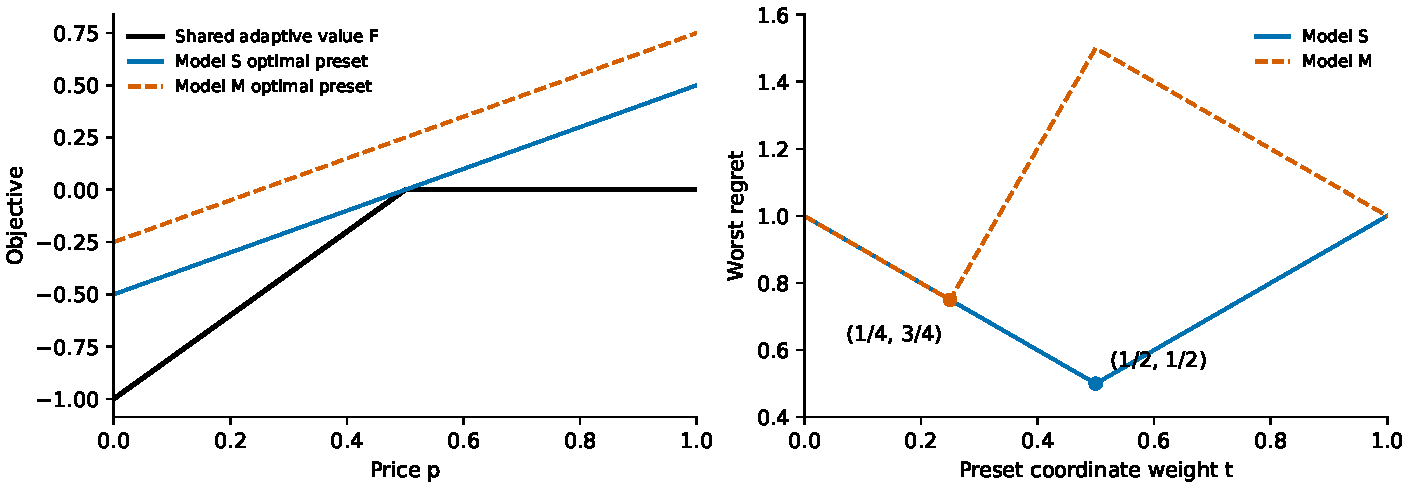
\includegraphics[width=\linewidth]{figures/structural.pdf}
\caption{The same fully adaptive curve permits different finite menus.
Left: the optimal realizable one-preset lines of Models S and M.
Right: their endpoint maximum regrets as a function of $t=u_1^2$.
The separation follows exactly from Proposition~\ref{prop:separation}.}
\label{fig:structural}
\end{figure}

\section{What the adaptive curve retains and loses}\label{sec:structure}
The separation in Proposition~\ref{prop:separation} raises quantitative
questions. How far can a curve-only relaxation underestimate menu regret?
When is it exact? Can additional globally optimal presets compensate for
its failure? We answer these questions using the slopes available on the
active spectral faces. The convex-geometric arguments apply more generally
to compact families of affine functions; the spectral model supplies an
explicit face test and finiteness of the exceptional prices.

\subsection{Three feasible families}
Identify an affine line with its coefficient pair and let
$\mathcal L=\{(\alpha(P),c(P)):P\in\Gr\}$, a compact subset of $\R^2$.
Let $\mathcal G\subseteq\Gr$ contain every preset that attains $F(p)$ at
some $p\in[0,B]$, including every choice at ties. This set is compact:
it is the projection of the closed optimality relation in
$\Gr\times[0,B]$. Write $E_K^{\mathcal G}$ for the menu optimum restricted
to $\mathcal G$, and $\overline E_K$ for the optimum when each preset line
can be any member of $\operatorname{conv}\mathcal L$. The latter is a
mathematical relaxation; a convex combination of effective lines need not
be realizable by a projector. The lower envelope remains $F$. Compactness
ensures attainment of all three optima, and
\begin{equation}\label{eq:threefamilies}
 \overline E_K\le E_K\le E_K^{\mathcal G}.
\end{equation}

The geometric statements below hold for any nonempty compact coefficient
set $\mathcal L\subset\R^2$, with presets interpreted as its elements and
$F(p)=\min_{(\alpha,c)\in\mathcal L}(\alpha+pc)$. Convexity of
$\mathcal L$ is not assumed. The spectral content is the realization of
the sharp examples, the explicit active-face formula, and finiteness of
the exceptional set. In particular, these results do not assert a new
general scalarization or convex-duality principle.

For $a<b$ define the curve-only endpoint value
\begin{equation}\label{eq:curveoracle}
 D(a,b)=\max_{p\in[a,b]}
 \{F(p)-F(a)-(p-a)s\},\qquad s=\frac{F(b)-F(a)}{b-a}.
\end{equation}
For an interior price define the compact set of available optimal slopes
\begin{equation}\label{eq:slopeset}
 S(p)=\{c(P):J(P,p)=F(p)\}.
\end{equation}
The right and left derivatives of the compact affine envelope are
$F'_+(p)=\min S(p)$ and $F'_-(p)=\max S(p)$, respectively. One way to
see the right-derivative identity is to compare $F(p+h)$ with each
minimizing line at $p$, then take a convergent subsequence of minimizing
lines at $p+h$ as $h\downarrow0$. The reverse inequality follows from
optimality at $p$. The left identity follows in the same way. Thus the
superdifferential is $[\min S(p),\max S(p)]$.

\begin{lemma}\label{lem:relaxation}
$D(a,b)$ is the exact endpoint minimax value for
$\operatorname{conv}\mathcal L$. An attaining relaxed line is either a
globally optimal preset line or a convex combination of two preset lines
that are globally optimal at the same interior price.
\end{lemma}
\begin{proof}
Every relaxed line lies above $F$. Its regret relative to the chord at
any price is a convex combination of its two endpoint regrets, giving
$D(a,b)$ as a lower bound. Maximize $F(p)-sp$ at $p_*$. If
$a<p_*<b$, then $s\in[\min S(p_*),\max S(p_*)]$. Choose two optimal
lines whose slopes bracket $s$ and mix them to have slope $s$. They agree
at $p_*$, so the mixed line has both endpoint regrets equal to $D(a,b)$.
If $p_*=a$, select a minimizing line at $a$ of smallest slope. The
right-derivative optimality condition makes its slope at most $s$, and
its regret at $b$ is at most its regret at $a$. If $p_*=b$, use the
largest minimizing slope and the left-derivative condition. The same
argument uses the appropriate one-sided derivatives at $0$ and $B$.
\end{proof}

The acceptable set of a relaxed line is again an interval. Consequently
Theorem~\ref{thm:greedy}, with $D$ in place of $e$, computes
$\overline E_K$ from $F$ alone in exact arithmetic. It computes a lower
bound on the realizable menu problem, with the following sharp comparison.
This is a statement about values and covering intervals: recovery of an
actual projector still requires the model's active-face information.

\begin{theorem}\label{thm:factor}
For every $K\ge1$,
\begin{equation}\label{eq:factor}
 \overline E_K\le E_K\le E_K^{\mathcal G}\le2\overline E_K.
\end{equation}
The constants in $E_K\le2\overline E_K$ and
$E_K^{\mathcal G}\le2E_K$ cannot be decreased uniformly over the spectral
models and budgets. Sharpness already occurs in the limit with $K=1$.
\end{theorem}
\begin{proof}
An optimal relaxed menu supplies a partition into at most $K$ segments,
each served by one relaxed line at tolerance $\overline E_K$. Such a
partition is obtained from its closed interval cover as in
Theorem~\ref{thm:greedy}. On a segment $[a,b]$ choose any globally
optimal preset at $q=(a+b)/2$. Its two nonnegative endpoint regrets sum to
\[
 2F(q)-F(a)-F(b)\le2\overline E_K,
\]
because the covering relaxed line lies above $F(q)$ and its endpoint
regrets are at most $\overline E_K$. Each endpoint regret is therefore
at most $2\overline E_K$, and convexity extends this bound to the segment.
One such preset per segment proves the last inequality. The other
inequalities are inclusions of feasible families. The next example proves
sharpness.
\end{proof}

\paragraph{A continuum of indistinguishable curves.}
Extend Model M by taking $C_1=2I$ and $C_2=\diag(\kappa,0)$ for
$\kappa>2$, retaining $A=\diag(1,0)$, $r=1$, $B=1$, and zero overheads.
For every $\kappa$,
\begin{equation}\label{eq:kappa}
 F(p)=\min(-1+2p,0),\qquad
 \overline E_1=\tfrac12,\quad
 E_1=1-\kappa^{-1},\quad E_1^{\mathcal G}=1.
\end{equation}
Indeed, with $t=u_1^2$ the endpoint regrets are $1-t$ and
$\min(2-t,(\kappa-1)t)$. For $t\le2/\kappa$ their maximum is minimized
at $t=1/\kappa$, with value $1-1/\kappa$. For $t\ge2/\kappa$ its
minimum is $1$. For $p>0$ the only globally optimal projectors are the
appropriate coordinate projectors, including both at $p=1/2$; at $p=0$
only the first coordinate is optimal. The relaxed value follows from
\eqref{eq:curveoracle}. Hence
\[
 \frac{E_1}{\overline E_1}=2-\frac2\kappa\longrightarrow2
 \quad(\kappa\to\infty),\qquad
 \frac{E_1^{\mathcal G}}{E_1}=\frac{\kappa}{\kappa-1}
 \longrightarrow2\quad(\kappa\downarrow2).
\]
Also $E_1^{\mathcal G}=2\overline E_1$ throughout the family. The same
curve realizes every value of $E_1$ strictly between $1/2$ and $1$.
Common positive definite shifts preserve the regrets. At $\kappa=2$
the optimal face at $p=1/2$ contains every projector, so the limiting
claim does not assert continuity of the restricted feasible family.

The factor-two argument is the elementary two-objective weighted-sum
bound applied to endpoint regrets. Weighted scalarization and limitations
of supported solutions have a substantial approximation literature
\cite{bazgan2022,helfrich2024}; we do not claim that principle as new. Here its role is
to quantify the information loss in Proposition~\ref{prop:separation},
with sharp examples inside the specified spectral model.

\subsection{An exact criterion on active slopes}
Call $p\in(0,B)$ a \emph{slope-gap price} if
$S(p)\ne[\min S(p),\max S(p)]$. This definition concerns missing slopes,
not merely nondifferentiability: a corner can have every intermediate
slope available from an optimal projector.

\begin{theorem}\label{thm:exactness}
The identity $e(a,b)=D(a,b)$ holds for every $0\le a<b\le B$ if and
only if there are no slope-gap prices in $(0,B)$. In that case
\begin{equation}\label{eq:exactmenus}
 E_K=E_K^{\mathcal G}=\overline E_K\qquad(K\ge1).
\end{equation}
\end{theorem}
\begin{proof}
If every $S(p)$ fills its interval, the interior construction in
Lemma~\ref{lem:relaxation} uses one actual globally optimal preset of
slope $s$. Its boundary construction already uses one preset. Thus
$e(a,b)=D(a,b)$ with a globally optimal realizing preset on every
segment. Applying this to an optimal relaxed cover proves
\eqref{eq:exactmenus}.

Conversely let $s$ be a missing slope at $p_*\in(0,B)$. Compactness of
$S(p_*)$ implies
$l:=F'_+(p_*)<s<u:=F'_-(p_*)$. Fix
$R>(u-s)/(s-l)$. For small $h>0$ set $a=p_*-h$. The chord slope
from $a$ to $p_*$ tends to $u>s$, whereas the chord slope from $a$ to
$p_*+Rh$ tends to $(u+Rl)/(1+R)<s$. By continuity there is
$b\in(p_*,p_*+Rh)$ for which the chord slope is exactly $s$.
Concavity and $l<s<u$ make $p_*$ the unique maximizer of $F(p)-sp$.

Suppose an actual preset attained endpoint error $D(a,b)$. At $p_*$
the positive weighted average of its endpoint regrets equals
$J(P,p_*)-F(p_*)+D(a,b)\ge D(a,b)$. Since each endpoint regret is
at most $D(a,b)$, equality forces both regrets to equal $D(a,b)$
and $J(P,p_*)=F(p_*)$. Equal endpoint regrets force $c(P)=s$,
contradicting $s\notin S(p_*)$. Attainment on the compact projector
set therefore gives $e(a,b)>D(a,b)$.
\end{proof}

\paragraph{Computing the slope set from spectral faces.}
At an interior price let $\mathcal A(p)=\{L:F_L(p)=F(p)\}$.
For each $L\in\mathcal A(p)$ use the cutoff-face construction in
Theorem~\ref{thm:endpoint} to obtain its minimum and maximum costs
$c_{L,-}(p)$ and $c_{L,+}(p)$. Then
\begin{equation}\label{eq:unionfaces}
 S(p)=\bigcup_{L\in\mathcal A(p)}
 [c_{L,-}(p),c_{L,+}(p)].
\end{equation}
Every intermediate cost is realized by the explicit rotations in that
theorem. Moreover, a minimizing projector of an active site must have
that site among its cheapest sites: since $p>0$, a strictly cheaper site
would yield an objective below $F(p)$. Conversely, a globally optimal
projector minimizes at a cheapest active site. This proves
\eqref{eq:unionfaces}. The restriction $p>0$ is essential to this
argument; at zero price a tied site's raw cost need not be the
projector's effective cost.

In particular, a single site has no slope-gap prices, even at eigenvalue
collisions. Differentiability of $F$ throughout $(0,B)$ is another
sufficient condition, since then every $S(p)$ is a singleton. With
multiple sites, one tests whether the union in \eqref{eq:unionfaces}
fills its interval. A jump in an optimizing subspace alone does not
imply failure of the curve relaxation.

\begin{remark}
The equivalence concerns relaxation exactness on \emph{every subinterval}.
It is not a converse criterion for \eqref{eq:exactmenus} on a single
fixed domain, or for the optimality of supported presets alone. For
Model M on $[1/2-h,1/2+h]$, $0<h<1/4$, direct endpoint calculation
gives $e=e^{\mathcal G}=2h$ but $D=h$. Here $e^{\mathcal G}$ restricts
the endpoint problem to globally optimal presets. Thus that restriction
can be exact even when convexification strictly improves the objective.
\end{remark}

\subsection{A finite cost in additional presets}
\begin{theorem}\label{thm:repair}
If there are $q<\infty$ slope-gap prices in $(0,B)$, then
\begin{equation}\label{eq:repair}
 E_{K+\min(K,q)}^{\mathcal G}\le\overline E_K\le E_K
 \qquad(K\ge1).
\end{equation}
Without finiteness, $E_{2K}^{\mathcal G}\le\overline E_K$ still holds.
For the finite-dimensional spectral model, $q$ is always finite.
\end{theorem}
\begin{proof}
Partition an optimal relaxed cover into at most $K$ segments and replace
its line on each segment by an endpoint optimizer from
Lemma~\ref{lem:relaxation}. If a globally optimal preset realizes that
line, retain it. Otherwise its slope lies in a gap of $S(p_*)$ at an
interior maximizing price. Choose two globally optimal lines at $p_*$
whose slopes bracket the required slope. Their lower envelope is no
greater than their convex combination at every price. The two actual
presets therefore cover this segment at its relaxed tolerance.

Each replacement that needs two presets can be charged to a slope-gap
price strictly inside its segment. Distinct segment interiors are
disjoint, so each price is charged at most once. There are at most
$\min(K,q)$ extra presets. This is selection between two deterministic
presets after observing the price, not a randomized projector.

For finiteness, apply Rellich's analytic eigenvalue parameterization to
each affine symmetric pencil on an open interval containing $[0,B]$
\cite[Theorem~1.1]{barbarino2022}. Each $F_L$ is the minimum of the
finitely many analytic functions obtained by summing any $r$ of those
eigenvalue branches and adding $pd_L$. Consequently $F$ is the minimum
of a finite family of analytic functions. Discard identical functions.
Every pair then has finitely many zeros of its difference on the compact
interval $[0,B]$. Outside their finite union, the minimizing analytic
function is locally fixed, so $F$ is differentiable. A slope gap
requires nondifferentiability by \eqref{eq:slopeset}, proving finiteness.
No polynomial bound on $q$, or efficient exact enumeration of it, is
asserted.
\end{proof}

Let $N_{\rm rel}(\epsilon)$, $N(\epsilon)$, and
$N_{\mathcal G}(\epsilon)$ be the least menu sizes at tolerance
$\epsilon>0$ in the three families. They are finite, and
\begin{equation}\label{eq:cardinalityrepair}
 N_{\rm rel}(\epsilon)\le N(\epsilon)\le N_{\mathcal G}(\epsilon)
 \le N_{\rm rel}(\epsilon)+\min\{N_{\rm rel}(\epsilon),q\}.
\end{equation}
Thus the extra supported-menu budget is bounded independently of the
requested accuracy for each fixed spectral instance. The bound counts
exceptional prices, rather than the number of missing slope intervals
at one price. It can be conservative: different repairs may reuse a
preset. Some overhead is necessary: the family in \eqref{eq:kappa}
has $q=1$ and $E_1^{\mathcal G}=1>\overline E_1=1/2$, whereas its
two coordinate presets give $E_2^{\mathcal G}=0$. Thus the extra preset
cannot be removed uniformly even for $q=K=1$. We do not assert sharpness
of the additive $q$ term for every $q$ and $K$.

For $K>q$, \eqref{eq:repair} also gives
\begin{equation}\label{eq:asymptoticsandwich}
 \overline E_K\le E_K\le E_K^{\mathcal G}\le\overline E_{K-q}.
\end{equation}
If a positive asymptotic law $\overline E_K\sim cK^{-\alpha}$ has been
established for a particular curve, then both $E_K$ and
$E_K^{\mathcal G}$ have that same leading law. This transfers existing
scalar approximation results, such as suitable one-sided smooth-curve
laws~\cite{gaubert2011}; it does not establish a new exponent or assert
those regularity assumptions for every spectral instance. Piecewise
affine curves can instead admit a finite zero-regret menu.

\paragraph{Relation to representative-set approximation.}
Minimum-size convex Pareto approximation already distinguishes feasible
representatives from convex combinations~\cite{diakonikolas2008}; the
detailed treatment in \cite[Sections~5.2--5.3]{diakonikolas2011} also
exhibits loss from restricting representatives to extreme supported points.
That phenomenon is not new here. Nor is replacement by supporting pieces:
\cite[Lemma~2]{magnanti2012} gives a bounded-cardinality tangent replacement
for multiplicative scalar approximation. Our two-line replacement is the
corresponding elementary exposed-face construction for additive regret.
The refinement is to charge a replacement only at an interior price with
an unavailable active slope; disjoint covering intervals charge each such
price at most once. Combining this count with \eqref{eq:unionfaces} and
spectral finiteness gives the instance-wise additive overhead. It does not
improve the computational-complexity guarantees of those predecessors.
Appendix~\ref{app:comparison} makes the approximation criteria and the
relation to robust policy-count bounds explicit.


\section{Endpoint construction and global covering}\label{sec:construction}
For $a<b$, let $f_a=F(a)$, $f_b=F(b)$, and $s=(f_b-f_a)/(b-a)$.
Define $e_L(a,b)$ as the best maximum endpoint regret at fixed site $L$.
The following spectral reduction is a specialization of established
two-objective trace minimax methods~\cite{tantipongpipat2019,shen2026}.
We include recovery and the proof to specify exactly what our menu oracle needs.

\begin{theorem}\label{thm:endpoint}
For each site,
\begin{equation}
 e_L(a,b)=\max_{p\in[a,b]}
 \{F_L(p)-f_a-(p-a)s\}.                                     \label{eq:dual}
\end{equation}
An actual rank-$r$ projector attains this value, including at a repeated
cutoff eigenvalue. The minimum endpoint regret with free site choice is
$e(a,b)=\min_L e_L(a,b)$. Set $e(a,a)=0$.
\end{theorem}
\begin{proof}
For any fixed projector, the convex combination of its endpoint regrets
with weights $(b-p)/(b-a)$ and $(p-a)/(b-a)$ is its regret relative to
the chord at $p$. Minimizing that combination gives the right side of
\eqref{eq:dual} as a lower bound on the maximum endpoint regret.

Choose a scalar maximizer $p_*$. All minimizing projectors of
$H=-A+p_*C_L$ contain its eigenspace strictly below $\lambda_r(H)$
and choose the remaining $k$ dimensions within its cutoff eigenspace.
Compress $C_L$ to that tied eigenspace. If its eigenvalues are
$\mu_1\le\cdots\le\mu_q$, the minimum and maximum costs on the
minimizing face are the fixed contribution plus $d_L$ and respectively
$\sum_{j=1}^k\mu_j$ and $\sum_{j=q-k+1}^q\mu_j$. Denote them by
$c_-$ and $c_+$.

Every intermediate cost is attainable by a pure projector. Retain the
shared coordinates of the $k$-low and $k$-high eigenspaces of the compression.
Pair the remaining low and high coordinates, replacing each low column
$e_i$ by $\sqrt{1-t}\,e_i+\sqrt{t}\,e_j$. Disjoint supports keep the
columns orthonormal; their total cost is $(1-t)c_-+tc_+$.
This is an explicit recovery construction, not random selection between
two projectors. Tied-space recovery itself is prior art~\cite{shen2026}.

The right and left derivatives of the affine envelope $F_L$ at $p_*$ are
$c_-$ and $c_+$. At an interior maximum of \eqref{eq:dual},
$c_-\le s\le c_+$. Select the face projector with cost $s$; its two
endpoint regrets coincide with the dual value. At $p_*=a$, choose cost
$c_-\le s$: the regret at $b$ is no larger than at $a$. At $p_*=b$,
choose cost $c_+\ge s$ and reverse the argument. Equality follows in
all cases. Finally, each projector has a single cheapest site at both
endpoints, so minimizing over projectors and the finite site set commutes.
\end{proof}

The following interval-covering characterization is standard; compare
\cite[Section~4.2]{cardinal2025}. We include its compactness argument
because the preset set here is an implicit continuum.

\begin{theorem}\label{thm:greedy}
For $\epsilon\ge0$ define
\begin{equation}
 T_\epsilon(x)=\max\{y\in[x,B]:e(x,y)\le\epsilon\}.
\end{equation}
Starting at $g_0=0$, set $g_j=T_\epsilon(g_{j-1})$, with
$T_\epsilon(B)=B$. Then $E_K\le\epsilon$ if and only if $g_K=B$.
\end{theorem}
\begin{proof}
The acceptable prices for a preset form a closed interval, so two acceptable
endpoints are equivalent to acceptability on their whole interval. A
maximizing $y$ and its preset exist by compactness. Further, $T_\epsilon$
is nondecreasing: a preset covering $[x,T_\epsilon(x)]$ also covers
$[x',T_\epsilon(x)]$ if $x\le x'\le T_\epsilon(x)$; otherwise
$T_\epsilon(x')\ge x'>T_\epsilon(x)$.

Greedy success constructs a menu. Conversely, a feasible finite menu gives
a closed interval cover, from which a chain of at most $K$ overlapping
intervals connects $0$ to $B$. If its reachable endpoints are $x_j$,
then $x_j\le T_\epsilon(x_{j-1})$. Induction using monotonicity gives
$x_j\le g_j$, forcing $g_K=B$.
\end{proof}

For $\epsilon>0$ progress is uniformly positive unless all preset slopes
coincide. If they lie in $[c_{\min},c_{\max}]$, a price-optimal preset
at $x$ has regret at most $(c_{\max}-c_{\min})|y-x|$ at $y$.
Thus the covering needs finitely many steps for positive tolerance. When
all slopes coincide, one optimal preset suffices everywhere.
The theorem supports a monotone outer search for $E_K$, but is an exact-real
characterization, not a complexity guarantee for finite-precision nested searches.

\paragraph{Numerical construction.}
For each candidate tolerance, the implementation makes at most $K$ farthest
endpoint searches. Each uses bisection in price and Theorem~\ref{thm:endpoint}
to test the interval, returning a realized preset. An outer bisection searches
the regret tolerance. For $K=1$ it solves only the full-domain endpoint problem.
At a site, the scalar objective in \eqref{eq:dual} is concave; slope bisection
and face recovery give primal and dual estimates. A site is feasible as soon
as an actual preset upper estimate is at most $\epsilon$; exclusion requires
lower estimates above $\epsilon$ at every site. Near eigenvalues are grouped
only to propose a basis, whose actual primal objective is then evaluated.
Unresolved oracle gaps raise an error. The numerical outer-search lower
estimate is not a certified lower bound: ambiguous finite-precision decisions
and finite price resolution are handled by separate witnesses below.

\paragraph{Computational work.}
Let $N_\epsilon$ and $N_p$ be the numbers of outer tolerance and price
bisections, and let $T$ bound the spectral evaluations needed by a completed
site endpoint solve, including recovery. A conservative uncached work count
is $O(N_\epsilon K(1+N_p)mTn^3)$ with dense eigensolvers. Tolerance bisection
gives logarithmic $N_\epsilon,N_p$ in the respective search resolutions,
but a uniform accuracy-dependent bound for $T$ near arbitrary collisions
is not asserted. The implementation caps it and reports unresolved gaps.
Saved-witness verification uses $O(Kmn^3)$ dense arithmetic operations,
independently of the number of outer search queries. Its constants include
explicit interval products; verification is timed separately from optimization.

\section{Reuse and independently checkable bounds}
The outer construction produces many related endpoint queries. A stored
site-preset line $\alpha+pc_L$ bounds $e_L(a,b)$ from above by
\begin{equation}
 \max\{\alpha+ac_L-F(a),\alpha+bc_L-F(b)\}.                 \label{eq:cachedprimal}
\end{equation}
A stored value $F_L(q)$ gives a lower bound
$F_L(q)-F(a)-(q-a)s$ whenever $q\in[a,b]$. Minimizing the cached primal
bounds and maximizing eligible dual bounds can settle a feasibility query
without a new eigendecomposition.

A minimizing preset at $q$ also gives a supergradient $c_L$ of $F_L$.
If $c_L>s$, the supergradient inequality rules out scalar maximizers strictly
to the left of $q$; if $c_L<s$, it rules out those strictly to its right.
The cache therefore brackets subsequent scalar searches. These are standard
supporting-line principles. We compare slope bisection with Brent both
without this reuse and with increasingly complete reuse. Inverted numerical
brackets are discarded. Full eigensystems use a bounded cache of about
32 MiB; supported basis records require additional memory, which is reported.

\begin{proposition}\label{prop:certificate}
Suppose $K$ presets and a contiguous partition of $[0,B]$ have endpoint
regret at most $U$, assigning one preset to each segment. Suppose also that
$K+1$ increasing prices $x_0<\cdots<x_K$ satisfy, for every adjacent pair,
\begin{equation}
 \min_L\{F_L(q_{i,L})-\operatorname{chord}_{x_i,x_{i+1}}F(q_{i,L})\}
 >\ell,\qquad q_{i,L}\in[x_i,x_{i+1}].                    \label{eq:packing}
\end{equation}
Then $\ell<E_K\le U$.
\end{proposition}
\begin{proof}
Convexity extends each segment's endpoint upper bounds to the full segment.
The weak-dual part of Theorem~\ref{thm:endpoint} shows that no preset can
serve an adjacent witness pair at tolerance $\ell$. Nor can it serve a
nonadjacent pair, since its acceptable set is an interval. Hence each preset
serves at most one witness, and $K$ presets cannot serve $K+1$ witnesses.
\end{proof}

The verifier is separate from the optimizer. Stored binary64 matrices mean
their exact real values. A stored basis $U$ means its exact polar-normalized
subspace $Q=U(U^TU)^{-1/2}$; it need not be exactly orthonormal as stored.
Outward interval arithmetic encloses its objective traces and the branch
spectral sums. The verifier checks segment adjacency, endpoints, witness
ordering, all site inequalities, and the final gap. Appendix~\ref{app:interval}
gives the enclosure argument and arithmetic contract. The checked eigensolver
only proposes a basis for an enclosure; neither its nominal precision nor
the menu solver's stopping test is trusted as a certificate.

For ordinary numerical evaluation, all pairwise intersections of the menu's
effective affine lines, together with $0,B$, suffice to find its continuous
maximum regret. Between crossings the lowest line is fixed and its regret
is convex. The interval verifier avoids the need to certify those computed
crossings by checking the saved covering segments instead.

\section{Computational evidence in brief}\label{sec:evidence}
The experiments test the construction and its certificates; they do not
establish the structural theorems or a physical resource model.
Appendix~\ref{app:experiments} retains the protocols, all comparison tables,
stress cases, and failed development attempts. The original three dense
studies contain 402 timed runs and 134 saved-menu checks. Against hybrid
Brent with the same cached primal/dual decisions, the median ratio of
reference time to reuse time is $1.367$ across 20 declared cells; its range
is $[1.255,1.866]$. Specialized two-dimensional formulas are faster than
the general construction. These are implementation comparisons, not a
new worst-case complexity result.

The dense studies and dictionary references include 54 independently
replayed global certificate artifacts of width $10^{-5}$, counting repeated
controls. Separately, the sharp family \eqref{eq:kappa} has 12 outward
checks matching its exact formula to below $10^{-10}$. The other structural
diagnostics are numerical checks, not proofs.

The sparse confirmation uses 72 timed runs in 12 paired cells. Dense
partial eigensolves are faster at dimensions 128 and 256; the sparse
backend wins at dimension 512 with cell ratios $1.39$--$1.90$. Larger
scaling cases are single observations. Independent banded verification
certifies all 14 saved sparse grid menus, including dimension 4096, with
gaps below $1.01\times10^{-5}$. Four of those grids also have earlier
dense certificates: these counts describe artifacts, not additional
independent instances. Banded verification exploits limited bandwidth,
rejects unresolved pivots, and is timed separately from optimization.
No performance claim for arbitrary sparse matrices or GPU execution is made.

\section{Scope and conclusions}
The useful structure is a shared reward, a scalar nonnegative price, and
quadratic site costs for a fixed-rank subspace. It yields an exact-real
finite-menu characterization and permits finite independent witnesses.
The scalar adaptive curve determines a relaxation that can underestimate
realizable regret by a factor approaching two. Missing optimal slopes
characterize failure of this relaxation on subintervals. They occur at
only finitely many prices in each fixed spectral instance, and their
number bounds the additional globally optimal presets needed to repair
a relaxed menu. Thus finite-budget distinctions coexist with agreement
of positive power-law leading asymptotics. The active-face test identifies
cases where curve approximation is already exact, including every
single-site instance. Site-specific information is needed to resolve
the general realizability constraint, not in every special case.
Repeated endpoint queries benefit from reuse on the reported dense families,
although the advantage narrows against a fully warmed Brent reference and
reverses against specialized two-dimensional formulas.

The sparse extension tests partial eigensolves at matched accuracy and
extends independent outward verification to banded inputs. Its scope
is specific graph-plus-diagonal families; it does not establish performance
for arbitrary sparse matrices, very large dimensions, many resource
parameters, site-dependent task rewards, negative prices, or externally
measured resource models. Verified grid bounds exploit their bandwidth;
arbitrary sparse graphs may have excessive fill or inconclusive pivots.
Additional basis storage
can grow even when the spectrum cache is bounded. Numerical convergence
near spectral collisions is not a bit-complexity guarantee. The central contribution is consequently a structural characterization
of convexification for finite spectral menus, supported by a construction
with checkable solutions. The extra-preset count is instance-dependent;
neither an efficient exact enumeration of exceptional prices nor a uniform
small bound on their number is supplied.

\section*{Statements and declarations}
\paragraph{Data and code availability.}
The accompanying artifact contains source code, frozen protocols, raw runs,
saved menus, witness files, and solver-independent verification commands.
It also contains the source for regenerating the tables and figure. The
versioned artifact is publicly available at
\url{https://github.com/Jevintlie/finite-spectral-menus/releases/tag/v7}.

\paragraph{Funding.} This research received no external funding.
\paragraph{Competing interests.} The author declares no competing interests.
\paragraph{Author contributions.} Jevint Felixciano developed the research
questions, directed the methodological and experimental investigation,
participated in the mathematical analysis and validation, and developed and
reviewed the manuscript, with the AI assistance described below.

\paragraph{Author information and disclosure.}
AI assistance was used in
research planning, literature searches, mathematical drafting, implementation,
numerical analysis, and manuscript preparation. The author is responsible
for the scientific claims, proofs,
attribution, code, and submission declarations. No journal acceptance or
external peer review is implied by the internal verification record.

\appendix
\section{Computational protocols and complete results}\label{app:experiments}
\subsection{Design and reproducibility}
The original three comparisons use our Python implementations with dense full
eigendecompositions, one BLAS thread, and fresh model/cache state per timed
run. Random matrices are $XX^T/n+0.1I$ with independent standard-normal
entries in $X$; site overheads are independent uniform draws in $[0,0.5]$,
and $B=2$. Shapes $(n,r,m)$ are $(8,1,1)$, $(16,4,3)$, $(32,8,6)$,
$(64,4,3)$, and $(64,16,3)$. Each family uses two seeds and budgets $K=2,4$.
The two-dimensional mirror model is a separate development control.
We use objective, price, and endpoint tolerances $2\times10^{-6}$,
$2\times10^{-8}$, and $10^{-9}$, respectively. These are numerical search
settings, distinct from the final verified gaps.

The initial confirmation uses seeds 5100/5101, two methods, and three
repetitions (132 runs). The stronger-reference study uses new seeds
5400/5401, three methods, and three cyclically ordered repetitions
(198 runs). Plans and source hashes were saved before their respective
executions; these are local records, not externally registered protocols.
Model generation and file saving are excluded from timings; cache building,
search, recovery, and numerical continuous maximum evaluation are included.
Certificate generation and independent checking are separate costs.
Results use ratios of per-cell median times, excluding the mirror control
from the primary summaries. No sample was removed for unfavorable timing.
The recorded environment is Python 3.12.10, NumPy 2.5.2, SciPy 1.18.1, on
Windows 11 with an AMD Ryzen 7 5800H processor. Hardware and library details
accompany the artifact.

Independent menu checks use a separate eigenvalue evaluation, verify basis
orthogonality and segment partitions, and evaluate every affine crossing.
A 101-point price grid is only a secondary consistency check. The initial
and stronger studies have 44 and 66 independently checked saved menus,
respectively. All paired numerical losses agree within $5\times10^{-6}$.

\subsection{Stronger scalar references}
The first Brent reference includes endpoint-aware early decisions and actual
primal recovery, but does not reuse bounds across different endpoint queries.
Its median time divided by the reuse method's time is $2.810$ on the 20
new-seed cells, with range $[2.112,5.934]$. This is not the headline gain:
warming the reference makes the comparison substantially closer.

The stronger study compares cached slope bisection with (i) Brent bracketed
by cached slopes, and (ii) hybrid Brent using both those brackets and the
same cached primal/dual decisions. Both Brent references retain a checked
recovery fallback if their parameter convergence does not close the objective
gap; fallback time is charged. Table~\ref{tab:warm} reports the results.
The median ratios are $1.630$ for bracket-warmed Brent and $1.367$ for
hybrid Brent, with ranges $[1.375,2.033]$ and $[1.255,1.866]$.
No reuse slowdown occurs in these 20 declared $K=2,4$ cells. This supports
a modest implementation advantage in this regime, not universal superiority
of bisection over Brent or a claim about prior authors' measured performance.

A separate ablation holds slope bisection fixed and removes the supporting-line,
dual-sample, and bracket reuse while retaining the same cache for identical
spectral queries. It uses seed 5500 in each shape, $K=2,4$, three alternating
repetitions, and the mirror control (72 runs, 24 checked saved menus).
All numerical loss differences are below $5\times10^{-6}$. Over the ten
new-seed cells, the plain-to-reuse median time ratio is $4.220$, with range
$[2.756,7.378]$. This isolates the combined reuse mechanism; it does not
isolate each cached-bound type, and it is a weaker comparison than hybrid Brent.

\begin{table}[t]\centering
\caption{Stronger-reference study. Each row aggregates four cells (two seeds,
two budgets). Ratios are reference seconds divided by proposed seconds;
larger values favor reuse with slope bisection. Memory is retained spectrum
and sample storage, not process peak RSS.}\label{tab:warm}
\begin{tabular}{rrrrrr}
\toprule
$n$ & $r$ & Sites & Warm Brent & Hybrid Brent & Max. MiB\\
\midrule
8 & 1 & 1 & 1.920 & 1.810 & 1.7\\
16 & 4 & 3 & 1.917 & 1.571 & 14.0\\
32 & 8 & 6 & 1.630 & 1.330 & 52.4\\
64 & 4 & 3 & 1.456 & 1.330 & 42.8\\
64 & 16 & 3 & 1.470 & 1.330 & 79.9\\
\bottomrule
\end{tabular}

\end{table}

\subsection{Dictionaries and special cases}
The dictionary comparison selects presets over the continuous price domain,
rather than judging them only on a grid. Uniform dictionaries contain
every site's minimizing basis at 129, 513, 2049, or 8193 prices. Selection
uses the same interval-covering geometry restricted to those candidates.
An adaptive heuristic starts at three prices per site, refines around selected
samples, and adds all-site minimizers at the menu's current worst price,
for at most 20 rounds. It has no additional targeted tied-space recovery.
This is our adaptive reference, not a reproduction of a published strongest
possible sampling algorithm.

Ten cases include the mirror model with $K=1,2,4$, three new random models
(seed 5200) with $K=2,4$, and one commuting collision control with $K=1$.
Stopping uses a generous oracle-assisted target: the proposed menu's
numerical loss plus $10^{-5}$. The dictionary is given that target, but
not the proposed preset directions. All candidate construction, refinement,
and repeated selection work is charged cumulatively. Final endpoint upper
bounds are verified independently. The reference menus also have global
certificates of width $10^{-5}$. Comparing the verified upper bounds with
those global lower bounds gives gaps below $1.94\times10^{-5}$ for every
dictionary menu that meets its target.

Uniform dictionaries meet their target in 1 of 10 cases within the cap;
the adaptive heuristic meets it in 6 of 10. Table~\ref{tab:dictionary}
reports every case, including failures to attain the target. These are
single-run descriptive timings. Coarser dictionaries can be faster when
less accuracy is required; these capped tests do not refute sampling with
other refinement rules or collision recovery. The separate commuting control
has one-preset loss $1/2$, while sampled coordinate eigenbases give $1$.
Unlike Proposition~\ref{prop:separation}, that control depends on which
basis the eigensolver chooses at a tie and does not exclude all choices there.

\begin{table}[t]\centering\small
\caption{Dictionary screen: cumulative seconds and target attainment at the
stopping stage or cap. ``No'' is failure to reach the accuracy target, not a
software failure. Verification time is excluded for all methods.}
\label{tab:dictionary}\begin{tabular}{lrrrrrr}
\toprule
Case & $K$ & Reuse (s) & Uniform (s) & Met? & Adaptive (s) & Met?\\
\midrule
Mirror & 1 & 0.005 & 0.766 & No & 0.015 & Yes\\
Mirror & 2 & 0.174 & 0.928 & No & 0.491 & Yes\\
Mirror & 4 & 0.392 & 1.258 & Yes & 1.039 & Yes\\
n16\,r4\,s3 & 2 & 0.321 & 2.935 & No & 1.637 & No\\
n16\,r4\,s3 & 4 & 0.872 & 3.924 & No & 3.584 & Yes\\
n32\,r8\,s6 & 2 & 0.837 & 13.613 & No & 9.358 & Yes\\
n32\,r8\,s6 & 4 & 2.277 & 17.129 & No & 21.652 & Yes\\
n64\,r4\,s3 & 2 & 1.209 & 18.032 & No & 17.157 & No\\
n64\,r4\,s3 & 4 & 2.691 & 22.925 & No & 44.356 & No\\
Collision & 1 & 0.001 & 0.379 & No & 0.019 & No\\
\bottomrule
\end{tabular}

\end{table}

The original mirror example has
$A=\left(\begin{smallmatrix}1&0.6\\0.6&2\end{smallmatrix}\right)$,
$C_1=\diag(0.2,3)$, $C_2=\diag(3,0.2)$, and overheads $0,1$.
It admits an independent analytic angular endpoint construction.
At matched stopping resolution it is much faster than the general method
(Table~\ref{tab:special}). This limits the practical recommendation:
use specialized formulas when available. Development one-preset tests also
favor Brent on several smooth examples; no $K=1$ speed advantage is claimed.

\begin{table}[t]\centering
\caption{Specialized mirror solver versus general reuse, median seconds from
three repetitions. All numerical loss differences are below $5\times10^{-6}$.}
\label{tab:special}\begin{tabular}{rrr}
\toprule
$K$ & Analytic (s) & General reuse (s)\\
\midrule
1 & 0.0015 & 0.0042\\
2 & 0.0067 & 0.1652\\
4 & 0.0128 & 0.3772\\
\bottomrule
\end{tabular}

\end{table}

\subsection{Checks of the structural results}
The script \texttt{check\_structural\_theory.py} checks six values of
$\kappa$ in \eqref{eq:kappa}, each with and without a positive definite
shift. All 12 cases have optimizer-independent outward upper/lower bounds
of width below $10^{-10}$ matching the exact formula. A further 54 numerical
endpoint checks use dimensions $2,6,8$, ranks $1,2,4$, one or three sites,
three seeds, and three intervals per instance. They check the factor-two
bound and single-site equality; these are diagnostics, not interval proofs.
An exact one-site crossing and three short Model M intervals check the
distinction in the remark following Theorem~\ref{thm:exactness}.

A three-coordinate, three-site example has $A=\diag(2,1,0)$,
$C_1=\diag(3,8,8)$, $C_2=\diag(8,1,8)$,
$C_3=\diag(8,8,0)$, zero overheads, $r=1$, and $B=2$.
Its adaptive curve is $\min(-2+3p,-1+p,0)$, with slope gaps at
$p=1/2$ and $p=1$. The relaxed two-cover splits at $2/3$, with
endpoint error $1/4$ on both segments. Direct selection from the three
globally optimal coordinate presets gives two-menu loss $1/3$ and
three-menu loss zero. The numerical unrestricted two-menu construction
also gives $1/3$; this last numerical value is not used as a proof.
These examples illustrate conservative repair counts and the distinction
between convexification and restriction to supported presets.

\subsection{Verification, stress cases, and retained failures}
The 22 proposed menus in each confirmation study and the 10 dictionary
reference menus have independently replayed global upper/lower bounds of
width $10^{-5}$. These are 54 saved certificate artifacts, including repeated
mirror controls, not 54 distinct random problems. They prove bounds for
their exact binary64 instances under Appendix~\ref{app:interval}'s contract.
Certificate generation may fail and is not asserted to succeed for all inputs.

We checked 24 site SDP solves on 12 instances with CVXPY and Clarabel
(agreement within $2\times10^{-7}$); some SDP statuses
include the recorded \texttt{optimal\_inaccurate} status. Twelve orthogonal
rotation checks agree within $2\times10^{-9}$. Twenty analytic stress cases
cover exact and near crossings, scales $10^{-6}$ through $10^6$, an eightfold
tie with several ranks including full rank, and dimension one. Interval
primitive checks compare 600 scalar cases and 87 matrix entries with exact
fractions, 84 eigenvalues with 80-digit arithmetic, and 18 perturbed-basis
polar objectives with high-precision calculations. These checks support the
implementation; they are not formal software verification.

Two development failures are retained. An initial certificate generator
mistook a cached primal basis's source price for a dual witness price;
one out-of-range proposal was rejected by the verifier. A revised generator
proposes a separate in-range price for each site and pair, and all 22 cases
then pass. A dictionary run initially stopped on serialization of a NumPy
Boolean; the corrected version changes serialization only. Neither incident
is hidden by deleting its result directory.

\subsection{Partial spectra and sparse computation}\label{sec:sparse}
The preceding studies use full dense spectra. A separate extension stores
the input matrices in compressed sparse row format and computes a partial
spectrum through ARPACK, using SciPy's \texttt{eigsh} interface
\cite{scipyeigsh}. The initial request is $\min(n,\max(r+8,2r))$ vectors;
it expands when the returned boundary is too close to the rank cutoff.
QR and Rayleigh--Ritz refinement, residual checks, and a 32 MiB spectrum
cache accompany the same reusable endpoint search. Dense fallbacks are
explicitly recorded and disabled above $n=1024$. This is an implementation
of established sparse spectral methods, not a new eigensolver.

The comparison uses a dense \emph{partial}-spectrum LAPACK backend with
the same outer search and recovery. Both receive identical synthetic
positive-semidefinite matrices: independently weighted graph Laplacians
plus positive diagonal terms. Edge weights lie in $[0.05,0.25]$, reward
diagonals in $[0.2,2]$, resource diagonals in $[0.1,1.5]$, and overheads in
$[0,0.15]$. The graph is a row-major grid of width $\lfloor\sqrt n\rfloor$,
possibly with an incomplete final row. These are computational test
families without a calibrated physical interpretation.

The initial sparse study stopped after 18 of 72 planned runs: both backends
failed all three repetitions of one rank-two case at $n=128$. A narrow
avoided eigenvalue crossing caused price bisection to reach binary64
resolution before meeting the $10^{-9}$ endpoint tolerance. The revised
implementation rotates the adjacent cutoff vectors to match the required
chord slope, evaluates the original primal objective, and accepts only
under the unchanged gap or decision criterion. The six failures and their
source snapshot are retained. This recovery is applied to both backends;
the failed study's seeds are thereafter treated as development data.

A new protocol uses fresh seeds 6400 and 6401, $n=128,256,512$,
$r=2,8$, two sites, and $K=2$. Three repetitions and two backends give
72 timed runs in 12 paired cells, with alternating method order, one BLAS
thread, and the preceding tolerances. Every saved menu is checked with
independent full dense eigenvalue evaluation at all affine-line crossings
and covering-segment endpoints. Those numerical cross-checks are distinct
from outward certificates. Table~\ref{tab:sparse} reports per-cell median
times; smaller instances need not benefit from sparse computation.

\begin{table}[t]\centering\small
\caption{Sparse confirmation. Times are medians of three runs in seconds;
the ratio is dense partial divided by CSR/ARPACK. A ratio above one favors
the sparse backend. Each row has two sites and two presets.}
\label{tab:sparse}\begin{tabular}{rrrrrr}\toprule
$n$ & $r$ & Seed & Dense partial & CSR/ARPACK & Ratio\\\midrule
128 & 2 & 6400 & 1.60 & 6.63 & 0.24 \\
128 & 2 & 6401 & 1.24 & 5.01 & 0.25 \\
128 & 8 & 6400 & 2.08 & 7.67 & 0.27 \\
128 & 8 & 6401 & 2.01 & 7.16 & 0.28 \\
256 & 2 & 6400 & 4.97 & 9.72 & 0.51 \\
256 & 2 & 6401 & 4.24 & 6.99 & 0.61 \\
256 & 8 & 6400 & 6.22 & 10.71 & 0.58 \\
256 & 8 & 6401 & 6.11 & 11.16 & 0.55 \\
512 & 2 & 6400 & 23.64 & 12.43 & 1.90 \\
512 & 2 & 6401 & 22.08 & 11.75 & 1.88 \\
512 & 8 & 6400 & 26.02 & 14.25 & 1.83 \\
512 & 8 & 6401 & 40.09 & 28.81 & 1.39 \\
\bottomrule\end{tabular}

\end{table}

All 72 confirmation runs completed, and all 24 saved menus passed the
independent numerical check. The median dense-partial/CSR runtime ratio
across the 12 cells is $0.564$. Its per-dimension medians
are $0.259$, $0.564$, and
$1.853$ for $n=128,256,512$, respectively.
Thus the small-instance overhead must be weighed against the measured
larger-instance behavior, rather than reporting only a favorable size.
The maximum difference between reported and independently evaluated losses
over confirmation and scaling menus is $2.5\times10^{-14}$.
The sparse runs in these two studies used 0 dense fallbacks.

Table~\ref{tab:sparse-scaling} extends the numerical screen to $n=4096$.
For the single $n=1024$ grid, the dense-partial/CSR ratio is $7.59$;
this one observation is not a repeated speedup estimate. Independent
ordered tridiagonal, full dense, and banded LAPACK calculations check path,
$n=1024$ grid, and $n=4096$ grid menus, respectively. The banded check uses
the known grid bandwidth, not the ARPACK proposals.

Outward verification and standalone replay also succeed for the four
$n=128$ CSR grid menus and all four path menus in the scaling screen,
each with a global bound width $10^{-5}$ to displayed precision. The grid certificates
use dense arithmetic; the path certificates use the tridiagonal verifier.
The banded verification study below extends certification to the larger grids.
Recorded array storage includes all cached preset bases, which can exceed
the spectrum-cache budget; it excludes transient solver workspaces and
Python overhead and is not a peak-memory measurement.


Partial eigenpair residuals do not establish extremal ordering or complete
cutoff multiplicity. The grid results therefore use separate ordered
spectral checks, with outward dense verification on selected tractable
cases. For paths, an outward Sturm-count verifier certifies ordered
eigenvalue sums without a dense matrix, using classical tridiagonal
inertia\cite{demmel1993}. Appendix~\ref{app:sturm} gives the argument.
The descriptive larger-instance screen also compares paths against a
specialized tridiagonal LAPACK solver; general CSR performance should not
be inferred from beating an unnecessarily dense path implementation.

\begin{table}[t]\centering\small
\caption{Descriptive scaling screen: one solve per method and case,
$r=2$, two sites, $K=2$. These are single observations, not repeated
confirmation estimates. Retained memory counts input, spectrum-cache peak,
and final basis-sample arrays, not peak process RSS.}
\label{tab:sparse-scaling}\begin{tabular}{lrlrr}\toprule
Graph & $n$ & Backend & Seconds & Retained MiB\\\midrule
Path & 1024 & CSR/ARPACK & 17.09 & 60.6 \\
Path & 1024 & Tridiagonal & 5.03 & 54.5 \\
Path & 4096 & CSR/ARPACK & 64.34 & 140.8 \\
Path & 4096 & Tridiagonal & 23.98 & 140.8 \\
Grid & 1024 & Dense partial & 134.49 & 83.6 \\
Grid & 1024 & CSR/ARPACK & 17.73 & 59.8 \\
Grid & 4096 & CSR/ARPACK & 189.80 & 356.3 \\
\bottomrule\end{tabular}

\end{table}

\paragraph{Outward verification of every CSR grid menu.}
A further verification study certifies all 12 CSR confirmation menus and
both CSR grid scaling menus, through $n=4096$, using interval $LDL^T$
elimination in band storage. All 14 certificates pass standalone replay,
with global gaps below $1.01\times10^{-5}$ (Table~\ref{tab:banded}).
This strengthens the preceding numerical checks without changing any
optimizer, saved menu, or isolated runtime measurement.

An initial binary64 interval implementation rejected a rank-eight witness
because its eigenvalue brackets became too wide to prove exclusion. That
attempt is retained. The revised verifier retries unresolved counts at
$n\le512$ with directed 50-digit decimal intervals; 57 counts use this
path. Both larger grid cases need only outward binary64 arithmetic.
The final checker independently encloses ordered eigenvalue sums and actual
polar-orthonormalized projectors; it imports no menu solver. Six CPU
processes check independent price/site pairs. These parallel verification
times are separate from the isolated optimization study.

For half-bandwidth $b$, each unpivoted inertia count uses $O(nb^2)$ work
and $O(nb+b^2)$ storage. The grid has $b=\lfloor\sqrt n\rfloor$;
at $n=4096$, packed input bands occupy about 6.1 MiB and an interval factor
about 4.1 MiB per worker, excluding temporary arrays and process overhead.
This is an advantage of band structure, not a guarantee for arbitrary
sparse graphs. Ambiguous pivots cause rejection; high bandwidth can erase
the storage benefit. Appendix~\ref{app:sturm} gives the factorization
argument and arithmetic assumptions.

\begin{table}[t]\centering\small
\caption{Independently replayed outward certificates for CSR grid menus.
Decimal counts record successful higher-precision inertia retries;
the displayed gap column is rounded. All unrounded gaps are below
$1.01\times10^{-5}$.}
\label{tab:banded}\begin{tabular}{rrrrr}\toprule
$n$ & Menus & Half-bandwidth & Decimal counts & Max. gap / $10^{-5}$\\\midrule
128 & 4 & 11 & 18 & 1.000029 \\
256 & 4 & 16 & 26 & 1.000031 \\
512 & 4 & 22 & 13 & 1.000031 \\
1024 & 1 & 32 & 0 & 1.000008 \\
4096 & 1 & 64 & 0 & 1.000008 \\
\bottomrule\end{tabular}

\end{table}




\section{Outward bounds for eigenvalues and actual subspaces}\label{app:interval}
The arithmetic contract interprets each binary64 input as an exact real
number. Elementary $+,-,\times,/$ operations are widened using
\texttt{nextafter}; matrix products use explicit interval sums, not
uncontrolled BLAS reductions. Correctly rounded IEEE-754 binary64 elementary
operations and gradual underflow are assumed. Nonfinite intermediates or
failed rank checks preclude certification. There is no formal proof-assistant
verification or independent external audit of the code.

For an exact symmetric $H=-A+pC_L$, an approximate eigensystem $V,D$ is
only a proposal, with $D$ sorted. Interval products enclose
$G=V^TV$ and $M=V^THV$. Let $\eta\ge\|G-I\|_2<1$ and
$\rho\ge\|M-D\|_2$, obtained from absolute row-sum bounds for the
enclosed symmetric matrices. The generalized Rayleigh quotient differs from
the Rayleigh quotient of $D$ by at most
\begin{equation}
 \delta=\frac{\rho+\|D\|_2\eta}{1-\eta}.                  \label{eq:delta}
\end{equation}
Indeed $x^TGx\ge(1-\eta)\|x\|^2$; subtracting the two quotients and
bounding the residual numerator gives \eqref{eq:delta} uniformly in $x$.
Since $\eta<1$, $V$ is invertible. Generalized Courant--Fischer then yields
$|\lambda_j(H)-D_{jj}|\le\delta$ for every $j$. Summing the first $r$
enclosures and adding an interval for $pd_L$ encloses $F_L$.
Taking the minimum of all lower endpoints and the minimum of all upper
endpoints encloses $F$.

For a stored preset basis $U$, let
$\eta_U\ge\|U^TU-I\|_2<1$. Its polar basis
$Q=U(U^TU)^{-1/2}$ exists and
\begin{equation}
 \|UU^T-QQ^T\|_*=
 \sum_{j=1}^r|\sigma_j(U)^2-1|\le r\eta_U.
\end{equation}
Therefore an interval for $\tr(U^THU)$, enlarged by
$r\|H\|_2\eta_U$, contains the objective of the exact realizable
projector $QQ^T$. Adding $pd_L$ and subtracting the enclosure for $F$
gives endpoint regret bounds. On each saved segment the verifier chooses
one fixed site and uses its two endpoint bounds; convexity extends them
to the interval. Lower witnesses use outward arithmetic for every quantity
in \eqref{eq:packing}. This checks the final optimization gap without
running or importing the menu optimizer.

\section{Tridiagonal and banded outward verification}\label{app:sturm}
For tridiagonal $H=-A+pC_L$, write its diagonal as $a_i$ and
off-diagonal as $b_i$. At a real shift $x$, the recurrence
\[
 t_1=a_1-x,\qquad t_i=a_i-x-b_{i-1}^2/t_{i-1}
\]
gives an $LDL^T$ factorization of $H-xI$ whenever all pivots are nonzero.
By Sylvester's inertia law, the number of negative pivots equals the
number of eigenvalues strictly below $x$; this is the classical Sturm
count used in eigenvalue bisection\cite{demmel1993}. Our verifier encloses
every pivot by outward interval operations and accepts a count only if
each interval is finite and excludes zero. It rejects unresolved signs.

An approximate eigenvalue merely proposes a bracket. If certified counts
at $l,h$ satisfy $N(l)\le j-1$ and $N(h)\ge j$, then
$\lambda_j(H)\in[l,h]$. Summing the first $r$ enclosures and adding $pd_L$
encloses $F_L(p)$. This argument permits multiplicities and does not rely
on the ordering of approximate Ritz pairs. For a preset basis, evaluate
\[
 \tr(U^THU)=\sum_{k=1}^r\left(\sum_i a_iU_{ik}^2+
                   2\sum_i b_iU_{ik}U_{i+1,k}\right)
\]
by interval sums, then apply the polar-basis correction from
Appendix~\ref{app:interval}. An outward row-sum bound controls $\|H\|_2$.
The same saved segment and packing witnesses give global menu bounds.

No dense $n\times n$ array is required. Each successful Sturm count uses
$O(n)$ work, and the preset Gram calculation uses $O(nr^2)$ work.
These statements do not bound the number of bracket expansions or menu
search iterations. The implementation assumes the same elementary
arithmetic contract as the dense verifier and has not received an external
code audit.

For a symmetric matrix of half-bandwidth $b$, the same inertia argument
applies to unpivoted band $LDL^T$ elimination. At each step, if the pivot
interval excludes zero, interval arithmetic encloses the Schur update
$S_{ij}-v_iv_j/d$. Induction encloses the exact factorization, with no fill
outside the full band. Definite signs of all pivots certify the inertia.
A singular leading principal submatrix can prevent this calculation even
for a nonsingular matrix; the checker rejects such a case. One successful
count uses $O(nb^2)$ arithmetic operations and $O(nb+b^2)$ storage. A
banded eigensolver only proposes brackets, which are checked by counts.

The trace calculation extends to every stored off-diagonal band, and the
same polar correction gives an objective enclosure for an actual projector.
Outward pairwise addition trees are valid by induction on their nodes.
Independent branch-price checks can run in CPU processes without changing
these arguments.

Unresolved counts at $n\le512$ may be retried with directed 50-digit
decimal intervals. Exact conversion of each binary64 input and separately
downward/upward-rounded elementary operations enclose the same real matrix.
This path additionally assumes the correct directed rounding of Python's
\texttt{Decimal} implementation\cite{pythondecimal}. Nonfinite or zero-containing pivots still
cause rejection, and decimal underflow is trapped. No automatic decimal
fallback is used for larger inputs. These precision and bandwidth limits
are implementation choices, not unconditional convergence guarantees.


\section{Comparison with representative-set and policy-count results}
\label{app:comparison}
The affine coefficient representation clarifies both the connection to
prior work and the precise scope of the structural results. This section
does not claim that additive regret creates an unrelated optimization
problem: its supporting-line geometry is shared with established
representative-set methods.

\paragraph{Convex Pareto approximation.}
For a finite coefficient menu $Q\subset\mathcal L$,
\[
 \min_{z\in Q}\langle(1,p),z\rangle
 =\min_{z\in\operatorname{conv}Q}\langle(1,p),z\rangle.
\]
Thus taking a convex hull \emph{after selecting} the menu does not change
its value at any price. Allowing its $K$ selected coefficient points to
come from $\operatorname{conv}\mathcal L$, however, can change the optimum.
This is the distinction between the representative's feasibility and
convex evaluation of the selected set. In particular, use of convex
combinations in a Pareto-approximation definition does not itself distinguish
that literature from finite-menu evaluation.

Diakonikolas' detailed treatment~\cite[Chapter~5]{diakonikolas2011},
following~\cite{diakonikolas2008}, compares representatives selected from
a finite set with representatives allowed in its convex hull. Its
Section~5.2.2 explicitly recognizes the usefulness of points away from
the lower convex envelope. Theorems~5.3.3 and~5.3.5 concern multiplicative
approximation and cardinality with a weighted-optimization oracle;
Remark~5.3.6 distinguishes objective-space points from recoverable decisions.
Our separation example is a spectral realization of an established
obstruction. Our contribution concerns the all-subinterval exactness
criterion, pure spectral face recovery, and a repair count localized to
missing-slope prices, with every tied optimal preset retained in
$\mathcal G$. Merely changing multiplicative to additive error would not
by itself establish a substantive contribution.

\paragraph{Scalarization and replacement.}
Weighted-sum approximation factors and supported-solution limitations
are established in~\cite{bazgan2022,helfrich2024}. The factor-two proof
here is their elementary endpoint-regret counterpart; the sharp examples
place that loss inside the specified spectral model. Similarly,
Magnanti and Stratila~\cite[Lemma~2]{magnanti2012} replace multiplicative
piecewise-linear approximants with tangent pieces. Our refinement preserves
an additive tolerance and counts the particular prices at which a
realizable supporting line is unavailable. Rellich's theorem supplies
spectral finiteness; neither supporting-line replacement nor analytic
eigenvalue parameterization originates in this paper.

\paragraph{Robust policy counts.}
Finite-policy reductions based on convex representation appear in
\cite[Theorem~1]{hanasusanto2015} and~\cite{buchheim2017}.
Kurtz~\cite[Theorems~2 and~7]{kurtz2026} gives exactness and approximation
bounds for objectives concave in the uncertain parameter over a convex
uncertainty set, within a bounded integer-recourse setting. Here the
candidate projectors form a continuum and
$R(P,p)=\alpha(P)+pc(P)-F(p)$ is convex in price, so the required
concavity is absent in general.

Lifting to the cost vector $(1,p,-F(p))$ does not repair that mismatch:
its image is generally nonconvex, and convexifying it can change the menu
objective. For example, the two coordinate presets of Model M have zero
regret at every actual price. The lifted endpoint vectors are $(1,0,1)$
and $(1,1,0)$. At their midpoint $(1,1/2,1/2)$, both preset costs equal
$1/2$. Thus the supremum over the lifted convex hull is at least $1/2$,
although the original menu regret is zero. These policy-count results
therefore do not directly supply \eqref{eq:repair} through a minimax swap.
Conversely, our repair bound provides none of their algorithmic complexity
guarantees. Continuous hitting and covering, including the farthest-reach
characterization, already have explicit finite-adaptability treatments
\cite{cardinal2025}.


\bibliographystyle{plain}
\bibliography{references}
\end{document}
